\documentclass[MASTER.tex]{subfiles} 
\begin{document} 

 
  
  \huge
  \[ \mbox{Data Visualization with Python} \]
  
 
%       =======%
 
  
 \textbf{seaborn}
 
 \begin{figure}
  \centering
  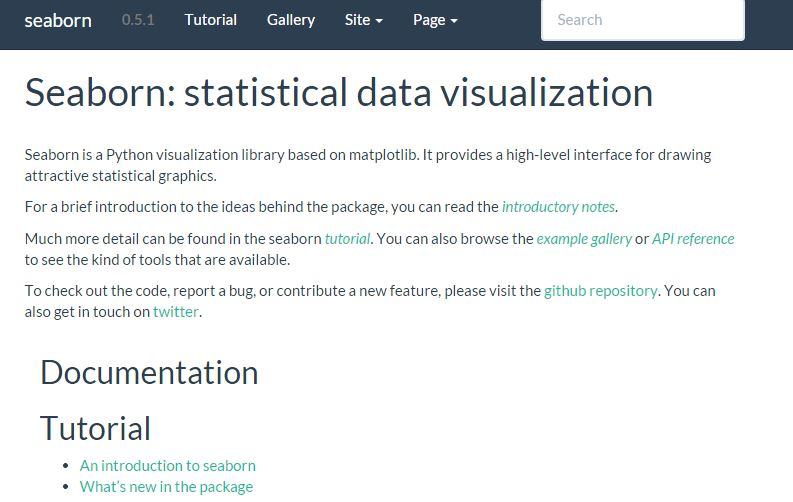
\includegraphics[width=1.05\linewidth]{seabornmain}
  
 \end{figure}
 
%       =======%
 
  
 \textbf{seaborn}
 
 \begin{figure}
  \centering
  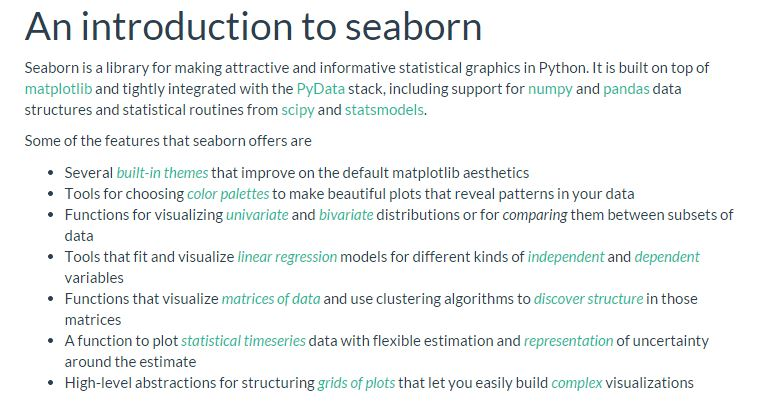
\includegraphics[width=1.05\linewidth]{seabornsiteinfo}
  
 \end{figure}
 
%      ======== %
 
  
 \textbf{seaborn}
 
 \begin{figure}
  \centering
  \includegraphics[width=0.80\linewidth]{seaborn1}
  
 \end{figure}
 
%       =======%

 
   
  \textbf{seaborn}
  
 \begin{figure}
  \centering
  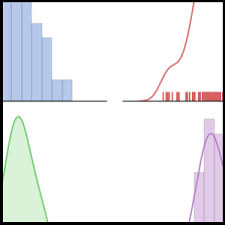
\includegraphics[width=0.80\linewidth]{seaborn2}
 \end{figure}
 
%       =======%

 
   
  \textbf{seaborn}
  
 \begin{figure}
  \centering
  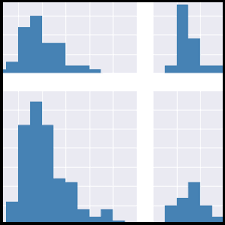
\includegraphics[width=0.80\linewidth]{seaborn3}  
 \end{figure}
 
%       =======%

 
   
  \textbf{seaborn}
  
 \begin{figure}
  \centering
  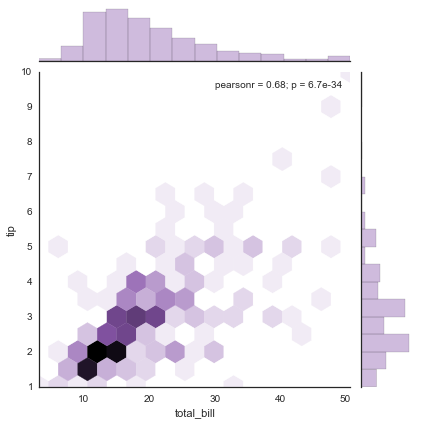
\includegraphics[width=0.80\linewidth]{seaborn4}
  
 \end{figure}
 
%       =======%

%      =====%
 
 \frametitle{Bokeh Data Visualization}
  \begin{figure}
\centering
\includegraphics[width=1.0\linewidth]{bokehlogo}
\end{figure}

 
%      =====%
 
 \frametitle{Bokeh Data Visualization}

\begin{figure}
\centering
\includegraphics[width=1.0\linewidth]{bokehplot}

\end{figure}
 
 
%      =====%
 
 \frametitle{Bokeh Data Visualization}
 \textbf{Bokeh Data Visualization}
  
   interactive graphics for the web
   designed for large data sets
   Designed for streaming data
   Native interface in pythin
   Fast javascript components
   DARPA funded
   v.01 relase imminent
  
 
 
\end{document}